\documentclass[11pt]{amsart} %amsart documentation: https://ctan.math.washington.edu/tex-archive/macros/latex/required/amscls/doc/amsclass.pdf
% The Proposal and Award Policies and Procedures Guide
% (PAPPG: https://www.nsf.gov/publications/pub_summ.jsp?ods_key=pappg)
% mandates, in Chapter 2, section B.2, that the main text should have a font size no less
% than 11 points for *most* typefaces (including Computer Modern Roman and Times (new) Roman).
% 
% Actually, Helvetica (a.k.a. Arial), Palatino and Courier New can drop
% to 10 point font size, according to the PAPPG,  but be aware:
% 10-point fonts (whatever the typeface) will promote reader fatigue.
% Reader fatigue never works to the author's advantage.
%
% This sample is set in 12 point type.
%

%choosing fonts: https://www.overleaf.com/learn/latex/Font_typefaces
\fontfamily{cmr}\selectfont %computer modern roman

\usepackage{amsmath,amsthm,amssymb,amscd}
\usepackage[numbers]{natbib}
\bibliographystyle{apj_small}
\usepackage{graphicx}
\usepackage{caption}
\usepackage{subcaption}
\usepackage{epsf}
\usepackage{cite}		% compress citations
\pagenumbering{gobble}		% Research.gov wants no page numbering
\tolerance9000
%
% The Proposal and Award Policies and Procedures Guide
% (PAPPG: https://www.nsf.gov/publications/pub_summ.jsp?ods_key=pappg)
% mandates, in Chapter 2, section B.2, that margins must be at least 1 inch in all directions.
%
\advance\paperheight1.00cm
\advance\textheight1.00cm
\advance\vsize1.00cm
\advance\topskip-0.5cm
\advance\voffset-0.5cm
%
\oddsidemargin0.15cm
\evensidemargin0.15cm
\textwidth16.1cm
%
%
\renewcommand{\footnotesize}{\small\spaceskip4pt plus1.5pt}

%Pagination - research.gov does this automatically see PAPPG II.B.1
%\advance\footskip1cm
%\pagenumbering{arabic}
%\usepackage{fancyhdr}
%\pagestyle{fancy}
%\lhead{}
%\chead{}
%\rhead{}
%\lfoot{}
%\cfoot{\thepage}
%\rfoot{}
%\renewcommand{\headrulewidth}{0pt}
%
\newtheorem{thm}{Theorem}[section]
\newtheorem{prop}[thm]{Proposition}
\newtheorem{cor}[thm]{Corollary}
\newtheorem{lemma}[thm]{Lemma}
\theoremstyle{definition}
\newtheorem{notn}[thm]{Notation}
\numberwithin{equation}{section}

\newcommand{\aj}{The Astronomical Journal}
\newcommand{\apj}{The Astrophysical Journal}
\newcommand{\apjl}{The Astrophysical Journal Letters}
\newcommand{\apjs}{The Astrophysical Journal Supplemental Series}
\newcommand{\aap}{Astronomy \& Astrophysics}
\newcommand{\aaps}{Astronomy \& Astrophysics Supplemental Series}
\newcommand{\mnras}{Monthly Notices of the Royal Astronomical Society}
\newcommand{\baas}{Bulletin of the American Astronomical Society}
\newcommand{\zap}{Zeitschrift für Astrophysik}
\newcommand{\prr}{Physical Review Research}
\newcommand{\prf}{Physical Review Fluids}
\newcommand{\sol}{\ensuremath{\odot}}
\newcommand{\RB}{Rayleigh-B\'{e}nard }
\newcommand{\grad}{\ensuremath{\nabla}}



\newcommand\Z{{\mathbb Z}}
\newcommand\Q{{\mathbb Q}}
\newcommand\R{{\mathbb R}}
\newcommand\C{{\mathbb C}}
\newcommand\F{{\mathbb F}}
\newcommand{\G}{{\mathcal{G}}}
\newcommand{\T}{{\mathcal{T}}}
\newcommand\Hom{\text{Hom}}
\newcommand\rank{\mathop{\text{rank}}}
\let\tensor=\otimes

\graphicspath{{./figures/}}

%AAPF:
%Project Description: Please note this section must include a separate section header labeled Broader Impacts and the heading must be on its own line with no other text on that line. The Project Description must be no more than ten (10) single-spaced pages in length, and it must include:
% -a coherent plan for research and education articulated to a level of detail suitable for an NSF grant proposal;
% -a detailed justification for the choice of host institution(s) that identifies collaborating scientist(s) and educational mentor(s), relates the proposed work to current research and educational efforts at the host institution(s), and describes available facilities and resources and the suitability of the host institution(s); and
% -a description of the proposer's long term career goals and role of this postdoctoral experience in achieving them.


%PAPPG: https://www.nsf.gov/publications/pub_summ.jsp?ods_key=pappg
\begin{document}
%\thispagestyle{fancy}


\centerline{\bf Postdoctoral Fellowship: AAPF:}
\centerline{\bf Building modern models of convection in massive stars}
\setcounter{section}{0}
\vskip-.7\linespacing
\section{Motivation}

Massive stars are the cornerstone of many fields of astrophysics.
Ionizing radiation from massive stars regulates star formation and the interstellar medium structure \citep{lancaster_etal_2021} and was important in the reionization of the early universe \citep{bromm_larson_2004}.
Massive stars end their lives in dynamic explosions which produce supernovae and observable high-energy transients \citep{heger_2003} and leave behind compact remnants like black holes and neutron stars \citep{abbott_etal_2018}.
A star's properties---ranging from its surface radiation field to the type of explosion that ends its life---depend intricately on its complex evolutionary history \citep{farmer_etal_2016}, which involves many uncertainties.
One key source of error in stellar modeling and evolution is the treatment of convection.


\textbf{Modern precision observations have revealed major theoretical shortcomings in models of stars and stellar convection.}
Asteroseismology and eclipsing binary studies reveal the need for larger convective cores than standard models produce \citep{johnston2021}.
\emph{Gaia} has provided exquisitely detailed HR diagrams of clusters, but modeled isochrones cannot reproduce the color and magnitude of observed populations along the main sequence \citep{gaia_2018}.
Kilometer-scale gravitational wave observatories (e.g., \emph{LIGO}/\emph{VIRGO}) are probing the populations of massive remnants \citep{abbott_etal_2018}, and convective mixing influences theoretical predictions of gaps in the remnant distribution \citep{vanson_etal_2022,farmer_etal_2019}.
Convection is a 3D turbulent process which adjusts a star's thermal structure and efficiently mixes chemical discontinuities, but is typically implemented in stellar evolution models using some form of the decades-old mixing length theory \citep[MLT,][]{bohmvitense_1958}, which has many shortcomings.
%Stellar models cannot explain our modern precision observations, and convection is at the root of many disagreements between models and observations.
\textbf{Disagreements between theory and observations demand new state-of-the-art models of convection informed by 3D simulations. }

The cores of massive stars ($M_* \gtrsim 1.1 M_\odot$) host convection, and the size of the convective core is a key uncertainty in massive star evolution.
Observations cannot be explained without larger cores than standard models produce, and convective boundary mixing (CBM) is often invoked to expand the core.
For example, in order to reproduce the observed population of eclipsing binaries, stellar models must employ a mass-dependent CBM \citep[see Fig.~\ref{fig:intro}, middle;][]{claret_torres_2019}.
Apsidal motion in binaries can be used to probe the density structure of stars \citep{rosu_etal_2022}, and these measurements suggest substantial CBM occurs.
When stars in stellar clusters are placed on the HR diagram, we observe wider main sequences than standard evolutionary models predict \citep{castro_etal_2014,higgins_vink_2019}, but introducing CBM aligns models with observed populations.
Finally, asteroseismology can now measure the internal radial distribution of mixing processes in stars; these measurements reveal extensive CBM outside of the convective core \citep{michielsen_etal_2019,pedersen_etal_2021}.
Combined, there is a large body of evidence suggesting that additional mixing is required at the core convective boundary of massive stars, but there are mass-dependent trends which have no theoretical explanation \citep{johnston2021}.
CBM is often treated as a free parameter.
Ad-hoc CBM prescriptions used in the literature produce core masses which vary by 70\% \citep{kaiser_etal_2020}, and these prescriptions must be finely tuned to match observations.
A unifying theory of CBM which reproduces observations self-consistently based on properties of stellar structure is desired.
Larger convective cores achieved by CBM have access to excess fuel, so it is impossible to accurately predict fundamental stellar properties like the star's lifetime, its pathway through the HR diagram, and the character of the remnant it leaves behind without improved CBM models.

\begin{figure}[t!]
     \centering
     \captionsetup{width=0.97\linewidth}
     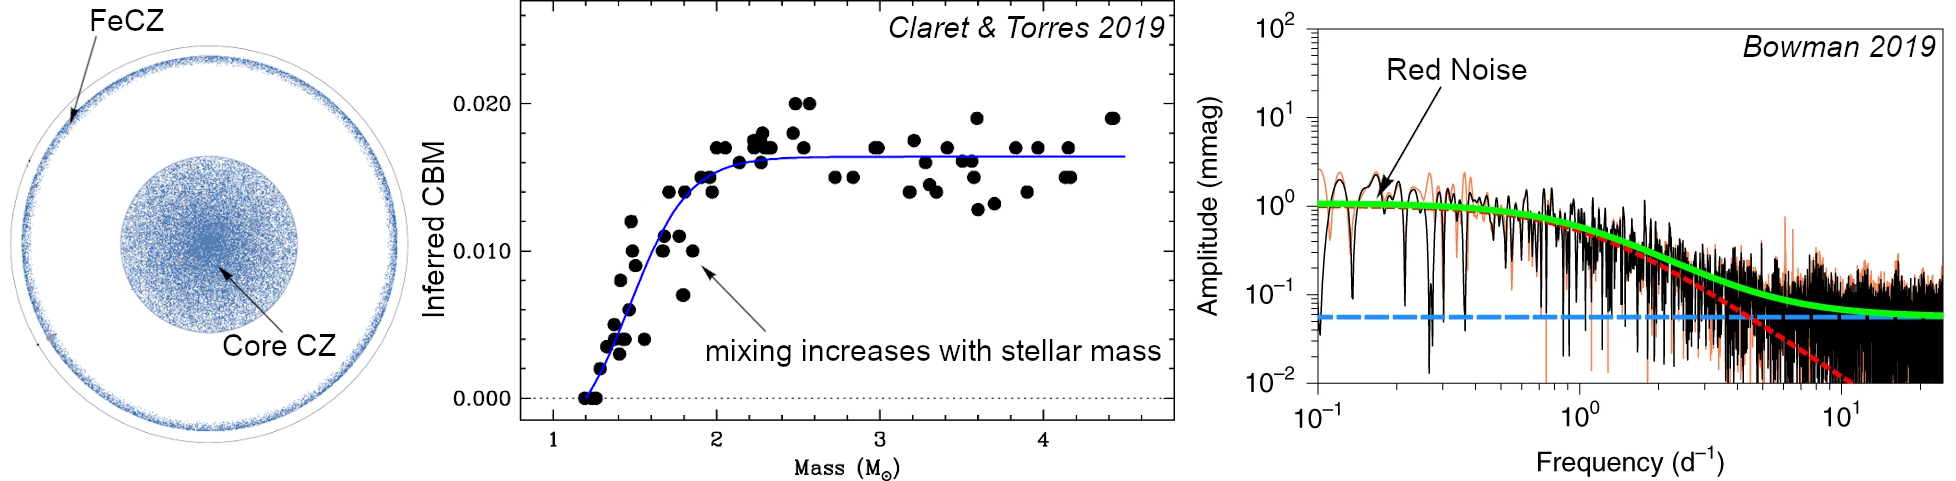
\includegraphics[width=\textwidth]{fig1.png}
        \caption{(Left) The structure of a massive star; shaded regions denote the core convection zone (core CZ) and iron convection zone (FeCZ) \citep{jermyn_etal_2022_atlas}.
        (Middle) Inferred convective mixing (y-axis) versus stellar mass for eclipsing binaries; note the strong mass dependence \citep{claret_torres_2019}.
        (Right) An amplitude spectrum of ``red noise'' in a hot, massive star; note the appreciable signal (black line) in excess of the noise floor (blue line) at low frequencies \citep{bowman_etal_2019}. 
        \label{fig:intro}}
\end{figure}

The surfaces of massive stars are dynamic.
Motions at the stellar surface broaden spectral lines in a phenomenon generally referred to as ``macroturbulence'' \citep{schultz_etal_2022b}.
A recent study of hot massive stars has also revealed a flat excess of power or ``red noise'' at low temporal frequencies \citep[see Fig.~\ref{fig:intro}, right;][]{bowman_etal_2019}.
Until recently, it was believed that the only convective engine in massive stars was the core convection zone (core CZ), but updates in opacity tables have revealed that massive stars have more convection zones than previously thought \citep[see Fig.~\ref{fig:intro}, left;][]{cantiello_etal_2009}.
In addition to core CZs, most massive stars have opacity-driven convective shells near their surfaces introduced by specific ionization states of hydrogen, helium, and iron.
The ``iron-bump'' convection zone (FeCZ) is of particular interest.
FeCZs are highly turbulent and the turbulence from these zones could produce macroturbulence and red noise \citep{cantiello_etal_2021, schultz_etal_2022, schultz_etal_2022b}.
Only a few simulations of FeCZs exist \citep{jiang_etal_2015}, so it is still unclear whether e.g., red noise is a manifestations of core gravity waves---in which case it can be used to probe stellar structure---or a manifestations of FeCZ turbulence.
Further simulations to characterize how FeCZs modify core-generated gravity waves and to understand the turbulent spectrum produced by these zones are required.

In addition to producing poorly characterized turbulent dynamics, FeCZs are highly radiation-dominated and the luminosity typically approaches the Eddington limit \citep{jermyn_etal_2022_atlas}.
In this extreme regime, MLT-based prescriptions produce density inversions which require ad-hoc and unphysical solutions to stably evolve stellar evolution models \citep{kohler_etal_2015}.
These effects combine to inflate the stellar radius, which in turn reduces the effective surface temperature; this temperature feeds directly into models of wind-driven mass loss \citep{yusof_etal_2013}.
The presence of an FeCZ therefore introduces uncertainty both into the thermal structure of a star and its mass loss history, which in turn affect the star's evolutionary track and remnant formation processes in a similar but orthogonal manner to core CZ CBM.

These puzzles demand models that go beyond the current state-of-the-art.
\textbf{The goal of this proposal is to build a next-generation set of 3D numerical simulations of convection in massive stars, which will answer the following questions:}
\begin{enumerate}
    \item How large are convective cores in massive stars?
    \item How does iron-bump convection affect observable waves and turbulence at the stellar surface?
    How does iron-bump convection affect the stratification of massive stars, and how does this affect the position of these stars on the HR diagram? 
\end{enumerate}

\newpage
\section{Focus I: Convective Boundary Mixing}
%Observations consistently demonstrate a need for improved models of convective boundary mixing (CBM) \citep{johnston2021}.
%Stellar models require an unexplained mass-dependent CBM to reproduce observed eclipsing binary populations  \citep{claret_torres_2019}.
%The amount of CBM used in stellar evolution models determines the main sequence width on the HR diagram and thus the stellar lifetime, luminosity, and effective temperature \citep{castro_etal_2014,higgins_vink_2019}. 
%Asteroseismology directly probes the results of CBM, revealing extensive mixing near convective core boundaries, and that \emph{both} entropy and chemical composition mix in a process called ``convective penetration'' \citep{michielsen_etal_2019, pedersen_etal_2021}.
%Models also require extra mixing in low mass stars with convective envelopes; lithium ignites at a greater depth than the estimated convective boundary, but observed lithium abundances suggest that convective motions reach the lithium ignition depth  \citep{pinsonneault_1997,binks_etal_2022}.




Observations demonstrate a need for improved models of convective boundary mixing (CBM) \citep{johnston2021}, and simulations also tell us that convection prefers larger cores than current models produce.
Simulations based on standard stellar models exhibit rapid turbulent entrainment at convective boundaries \citep{rizzuti_etal_2022}, but these simulations are rarely run for long enough for the size of the convection zone to saturate.
I recently performed simulations which demonstrated that energetically equilibrated convection zones can expand well beyond the Schwarzschild boundary, and also derived a prescription for the saturated size of the convection zone \citep[see Fig.~\ref{fig:cbm}, left;][]{anders_etal_2022a}.
When this prescription is applied in postprocessing to stellar models, we self-consistently reproduce the same CBM trend as is observed in eclipsing binaries \citep[see Fig.~\ref{fig:cbm}, middle;][]{jermyn_etal_2022_penconv}, which demonstrates exciting promise for our method.
However, my past simulations were performed, and this prescription was calibrated, using Cartesian simulation which employed the incompressible approximation; these assumptions are not valid for the cores of massive stars.

Stellar core convection is difficult to simulate.
Many codes require a ``cutout'' near $r = 0$, so flows cannot pass through the center of the star \citep{edelmann_etal_2019,horst_etal_2020,yadav_etal_2016}.
Core convection occurs at very low Mach numbers \citep[Mach $\sim 10^{-4}$;][]{jermyn_etal_2022_atlas,aerts_etal_2021}, and explicit timestepping techniques which require small timesteps to resolve the (fast) sound waves cannot resolve this low-Mach convection \citep{edelmann_etal_2021}. 
To avoid these restrictions, past studies have chosen to either employ the Anelastic approximation \citep[which is not thermodynamically valid for CBM studies;][]{brown_etal_2012,browning_2008,yadav_etal_2016} or boost the stellar luminosity \citep[which leads to excess CBM for unphysical reasons;][]{baraffe_etal_2021}.


\begin{figure}[t]
     \centering
     \captionsetup{width=0.97\linewidth}
     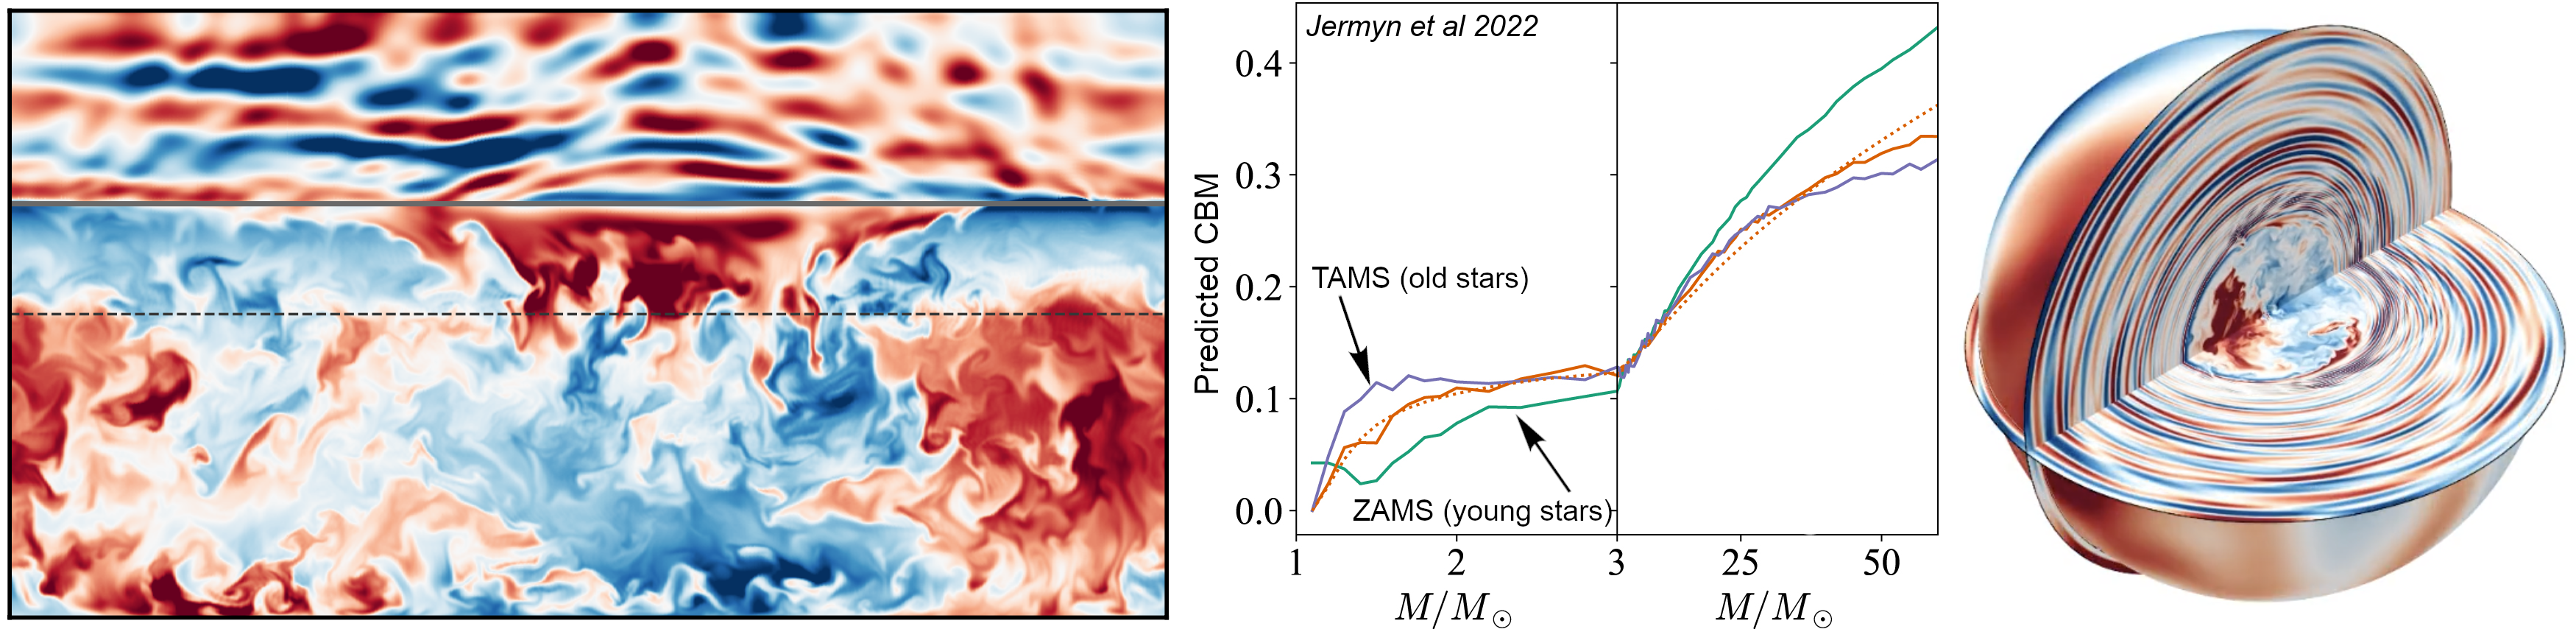
\includegraphics[width=\textwidth]{fig2.png}
        \caption{(Left) One of my \emph{Dedalus} simulations exhibiting penetrative convection; note the region between the Schwarzschild boundary (dashed line) and the measured convection zone boundary (solid line) where upflows which are hot below the Schwarzschild boundary turn cold \citep{anders_etal_2022a}.
        (Middle) Expected convective mixing in stars using a prescription from my Cartesian, incompressible simulations \citep{jermyn_etal_2022_penconv}. This figure can be compared to the middle panel of Fig.~\ref{fig:intro} by dividing by a factor of 10 due to different CBM measures being reported; a similar trend is observed at low mass.
        (Right) A \emph{Dedalus} simulation of core convection in a $40 M_{\odot}$ star that I ran using a preliminary version of the module I will use in the proposed work.
        \label{fig:cbm}}
\end{figure}

To address these modeling deficiencies, I will simulate core convection in massive stars using the \emph{Dedalus} \citep{burns_etal_2020} code.
My simulations will differ from past simulations, because they will include the full ``ball'' geometry of the convective core (including $r = 0$), they will employ the fully compressible equations without any luminosity boosting, and they will be allowed to evolve into thermal equilibrium; an example of one of these new state-of-the-art simulations is shown in the right panel of Fig.~\ref{fig:cbm}.
\emph{Dedalus} has the state-of-the-art ability to simulate flows that pass through the coordinate singularity at $r = 0$ in spherical coordinates \citep{vasil_etal_2019,lecoanet_etal_2019}.
I have accurately simulated very low Mach number flows in \emph{Dedalus} \citep{anders_brown_2017} without extreme timestepping restrictions by employing implicit-explicit (IMEX) timestepping techniques.
By implicitly timestepping the linear terms associated with sound waves while explicitly timestepping the nonlinear advective terms, we can stably and accurate evolve low-Mach core convection without luminosity boosting.
Regarding thermal equilibration, my previous CBM studies \citep{anders_etal_2022a,anders_etal_2022b} demonstrated that the structure of boundary mixing regions can take thousands of convective overturn times to saturate.
Fortunately, I have developed methods of ``accelerated evolution'' \citep{anders_etal_2018,anders_etal_2020}; these techniques rapidly equilibrate simulations while saving up to an order of magnitude in computational resources.
I will design these simulations with ease-of-use for the community in mind, and my simulation code and run scripts will be open source and accessible through Github and Zenodo.

All massive stars rotate rapidly \citep{jermyn_etal_2022_atlas}, but almost all CBM studies have neglected rotation because the parameter space of rotating convection is difficult to navigate.
In particular, it is the \emph{Rossby number} (Ro, the ratio of the rotational and convective timescales) which determines how rotation affects convective flows \citep{aurnou_etal_2020}.
Thus, while we know that the surface rotation rate of massive stars follows a simple relationship \citep{glebocki_gnacinski_2005,ramirezagudelo_etal_2013,nielsen_etal_2013}, a simulation of convection using the realistic rotation rate and realistic luminosity might produce convection with a different Ro than the star being modeled; this occurs because simulations are idealized representations of stars, but cannot achieve e.g., realistically small diffusivities.
I will first follow past work and avoid this difficulty by studying fictional \emph{non-rotating} stars; without rotation it is straightforward to increase the turbulence to state-of-the-art limits then extrapolate results into the astrophysical regime.
After establishing this non-rotating benchmark, I will study realistic stellar simulations with rotation to understand how rotation affects the amount of CBM in a star.

\emph{\underline{Task 1:}}
I will study CBM in spherical simulations with background stratifications based on MESA models of massive stars (as in Fig.~\ref{fig:cbm}, right).
In this first task, I will focus on simulations of non-rotating stars spanning the mass range $M_* = 1.1-40 M_{\odot}$.
I will in particular study the low-mass range from $1.1-3 M_{\odot}$, where observed ``extra mixing'' is a strong function of stellar mass \citep[][Fig.~\ref{fig:intro}, middle]{claret_torres_2019}, and compare these simulations to observations of eclipsing binaries.

\emph{\underline{Task 2:}} I will include rotation into my models to understand how the stellar rotation rate affects convective boundary mixing.
Rotation is theorized to reduce the extent of convective boundary mixing \citep{augustson_mathis_2019}.
In our current theory of CBM via convective penetration \citep{anders_etal_2022a} the mixing region's size decreases as the dissipation in the convection zone increases.
Rotation organizes flows into vortices with high dissipation rates which are aligned with the rotation axis \citep{julien_etal_1996}, so it would make sense for rotation to decrease the amount of CBM, but I will test this explicitly.

\textbf{\underline{\emph{Deliverable:}} The first 3D simulations of rotating core convection in massive stars that include the coordinate singularity at $\boldsymbol{r = 0}$, reach thermal equilibrium, do not boost the luminosity, and span the main sequence.}
These models will be used to create a 1D implementation of CBM, which I will then work to include in the 1D \emph{MESA} stellar evolution software instrument.
I will publish the fully compressible \emph{Dedalus} module used to create these simulations, giving the community an open-source tool for studying dynamics in massive stars. 




\section{Focus II: Optically Thick Iron-bump Convection}
%%%%%%%%%%%%%%%%%%%%%%%%%%%%%%%%%%%%%%%%%%%%%%%%%%%%%%%%%%%%%%%%%%%%%%
\begin{figure}[t!]
     \centering
     \captionsetup{width=0.97\linewidth}
     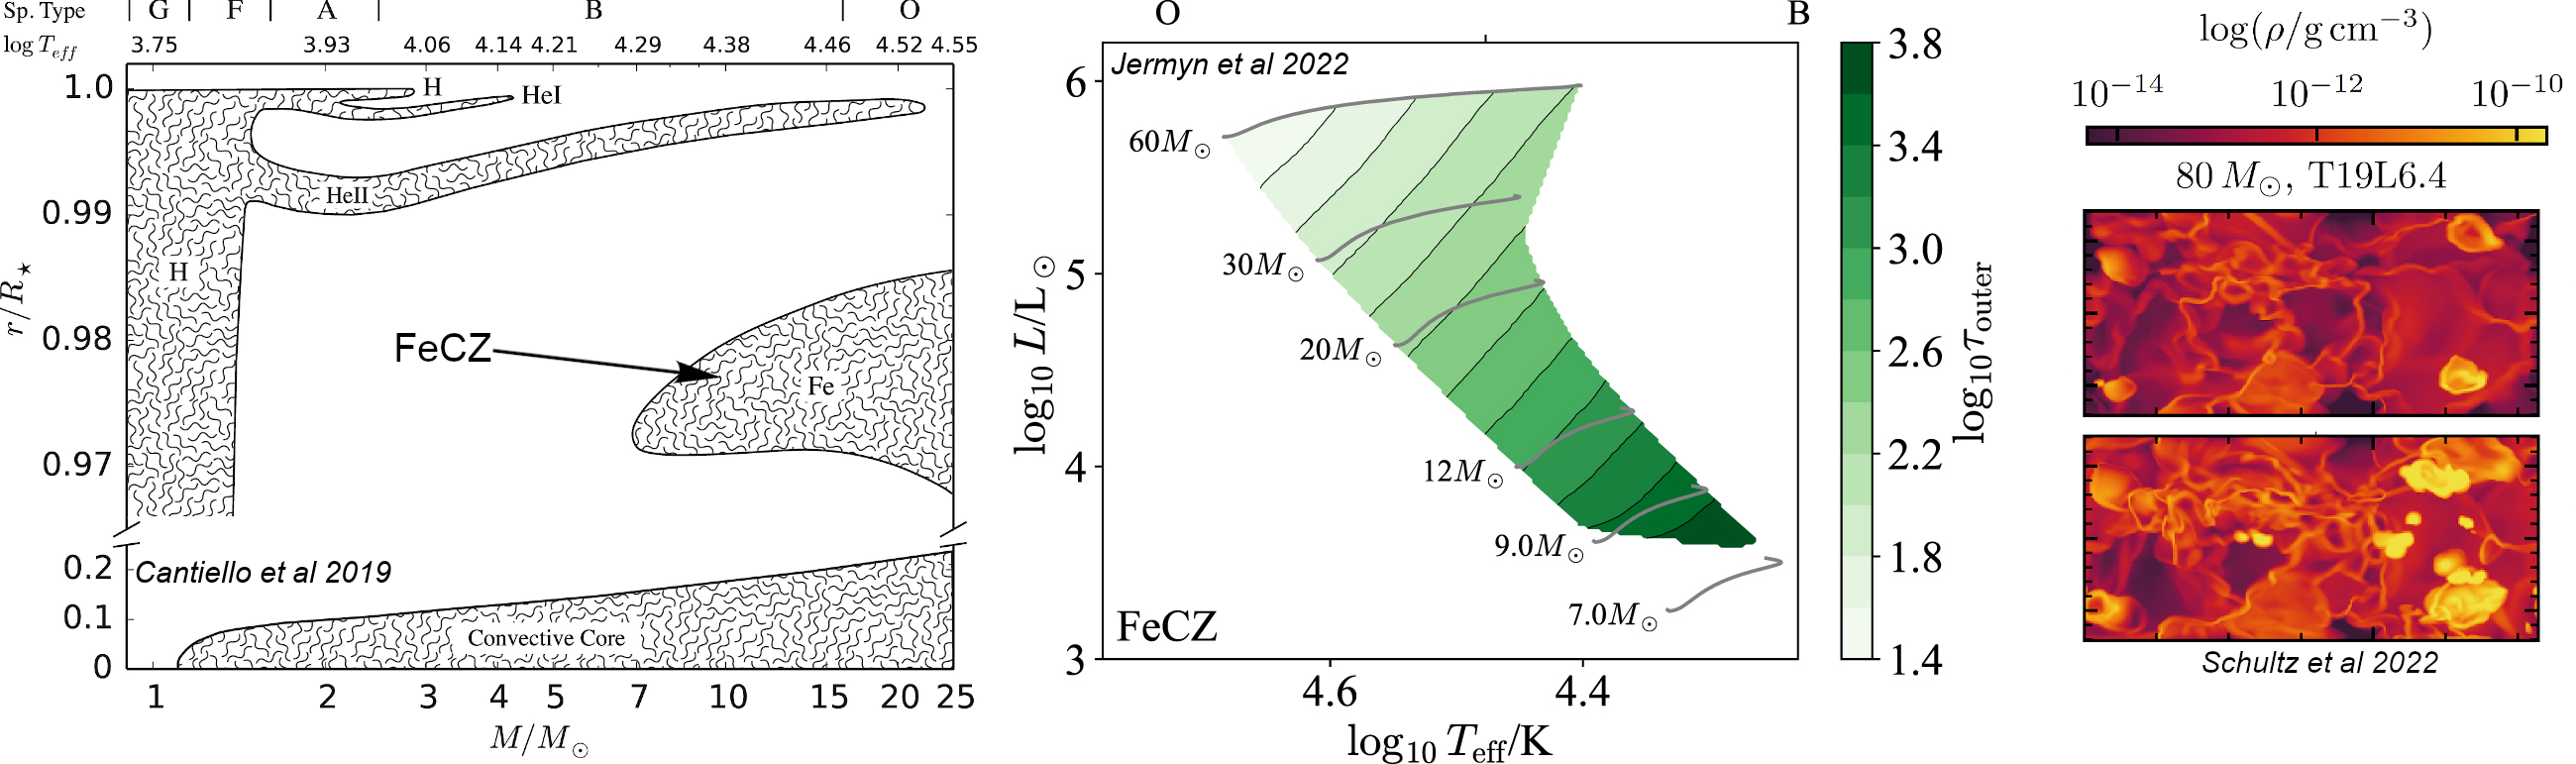
\includegraphics[width=\textwidth]{figures/fig3.png}
     \vspace{-0.7cm}
        \caption{
        (Left) Radial extent of convection zones as a function of stellar mass \citep[assuming metallicity $Z = 0.02$;][]{cantiello_braithwaite_2019}; note the appearance of the FeCZ for stars with $M \gtrsim 7 M_{\odot}$. (Middle) An HR diagram of main sequence massive stars; color denotes the optical depth from the FeCZ to the stellar surface and is always $\tau \geq 10^{1.4}$ for stars with $M_* \leq 60 M_{\odot}$  \citep{jermyn_etal_2022_atlas}. (Right) Dynamics in an FeCZ simulation in a 80 $M_{\odot}$ star; very high Mach number flows are seen, with densities at a fixed optical depth varying by four orders of magnitude \citep{schultz_etal_2022b}.
        \label{fig:fecz}
        \vspace{-0.5cm}}
\end{figure}

In addition to vigorous core convection, massive stars have opacity-driven convective shells in their envelopes \citep{cantiello_etal_2009}.
For stars with masses $\gtrsim 7 M_{\odot}$, iron opacity generates an ``Iron-Bump Convection Zone'' (FeCZ, Fig.~\ref{fig:fecz}, left).
Unlike convection zones at the photosphere of lower-mass stars (e.g., the Sun), these convection zones appear at high optical depths \citep[Fig.~\ref{fig:fecz}, middle;][]{jermyn_etal_2022_atlas}.
This regime of convection has not been the focus of extensive study, but can result in extreme dynamics (Fig.~\ref{fig:fecz}, right) which influence the stellar structure and evolution appreciably.

%FeCZs approach the Eddington luminosity limit \citep{jermyn_etal_2022_atlas}, and so can develop density and gas pressure inversions in stellar evolution models \citep{kohler_etal_2015}.
%These inversions are accompanied by inflation of the stellar surface 
%The stellar inflation accompanying these zones reduces the effective surface temperature which increases the efficiency of winds launched from the stellar surface, affecting the mass loss achieved by these stars and the subsequent stellar evolution \citep{smith_2014,kohler_etal_2015}.

Numerical simulations of FeCZs are extremely limited.
A few simulations of FeCZs for 40 and 80 $M_{\odot}$ stars were performed \citep{jiang_etal_2015} and studied in detail \citep{schultz_etal_2020,schultz_etal_2022,schultz_etal_2022b}.
%Extremely interesting dynamics were observed: the envelope above these zones is dynamic, and the high radiative efficiency despite convection is unlike core convection.
This high-Mach number convection creates a large dynamic pressure which is not included in the equation of state used in stellar evolution models.
This turbulent pressure will modify the thermal stratification of the stellar envelope and thereby affect the star's effective temperature, but the behavior of such a term must be calibrated using 3D hydrodynamical simulations before it can be self-consistently included in 1D models.
Unfortunately the full radiative hydrodynamic simulations of FeCZs which have been performed \citep{jiang_etal_2015} are extremely expensive, so it is unfeasible to use that tool to simulate many FeCZs across the HR diagram to calibrate this turbulent pressure.

Fortunately, since FeCZs occur in optically thick layers in many stars (Fig.~\ref{fig:fecz}, middle), the computationally cheap radiative diffusion approximation is valid and full radiative hydrodynamics are not necessary.
%As a result, it is possible to study much less expensive simulations that do not solve the full equations of radiative transfer but which do still include the iron opacity peak and high mach number flows.
Furthermore, FeCZs are very thin (aspect ratios $r / \delta r \sim 10^{1-3}$) and can be accurately modeled in a plane-parallel Cartesian domain \citep{jermyn_etal_2022_atlas}.
I will use \emph{Dedalus} to build on my past high-Mach number, fully compressible simulations \citep{anders_brown_2017} by including iron bump opacity effects in the radiative diffusion limit.
I will study a span of simulations varying stellar masses in the range $8-60\, M_{\odot}$ and ages ranging from the zero-age main sequence (ZAMS) to the terminal age main sequence (TAMS) to calibrate the turbulent pressure generated in FeCZs.

There is a current debate about whether the source of ``red noise'' on hot, massive stars \citep[Fig.~\ref{fig:intro}, right;][]{bowman_etal_2019} is gravity waves generated in the convective core or turbulence generated by FeCZs \citep{cantiello_etal_2021}.
Existing FeCZ simulations generate turbulent fields which could explain red noise signals as well as ``macroturbulence'' signals \citep{schultz_etal_2022,schultz_etal_2022b}.
Simulations of core generated gravity waves \citep{edelmann_etal_2019,horst_etal_2020} have also shown promising comparisons with red noise, but do not include the FeCZ, and so do not capture how the FeCZ modifies gravity wave signals from the core.
I will study how gravity wave signals generated below the FeCZ change as they pass through this turbulent convection zone.
I will include the stable radiative zones surrounding the FeCZ in my simulations and force a spectrum of gravity waves at the bottom boundary, then measure how these waves interact with and are modified by the turbulent convection in the FeCZ.

\emph{\underline{Task 3:}} I will use \emph{Dedalus} to study iron bump convection in Cartesian, optically thick simulations which span many stellar masses and ages.
I will measure how the turbulent pressure compares to the background pressure, and parameterize this for inclusion in 1D stellar evolution software instruments like \emph{MESA}.
I will work with experts in the \emph{MESA} community to include turbulent pressure into stellar evolution models, then I will generate a new suite of stellar evolution models to quantify how turbulent pressure affects the stellar radius, effective temperature, and other observable properties of these stars.

\emph{\underline{Task 4:}} I will use \emph{Dedalus} to simulate how an FeCZ modifies gravity waves generated by core convection.
These simulations will put the first constraints on whether or not gravity waves can pass through the FeCZ to be observable at the stellar surface.
Since gravity waves are one of the best tools for putting constraints on the interior structure of massive stars \citep{aerts2010}, it is critical to understand whether their signal is modified or blocked by FeCZs.
%The results of these simulations will help determine whether observers should look towards lower-metallicity, lower-mass stars where there are no opacity-driven convection zones for wave signals \citep{jermyn_etal_2022_window}.

\textbf{\underline{\emph{Deliverable:}} The first 3D simulations of iron-bump convection spanning the HR diagram, and the first 3D calibration of how the FeCZ affects asteroseismic gravity wave observations.}
These simulations will produce a 1D implementation of turbulent pressure generated by the FeCZ, which will improve stellar structure models of massive stars.
%These simulations will then be used to create the first experimental test of whether core generated gravity waves can pass through the turbulent motions in the FeCZ to be observed at the surface.
As with tasks 1-2, the \emph{Dedalus} simulation tools used to create these FeCZ simulations will be open-source, published, and widely accessible.

%%%%%%%%%%%%%%%%%%%%%%%%%%%%%%%%%%%%%%%%%%%%%%%%%%%%%%%%%%%%%%%%%%%%%%
\section{Educational Development: Partnership between KITP and SST}

At UCSB, the Center for Science and Engineering Partnerships (CSEP) runs the School for Scientific Thought (SST).
SST is a program for students in grades 9-12 which offers courses that meet for three consecutive Saturdays for three hours of instruction and 1 hour of networking or lab tour/panels over lunch each Saturday (12 hours total).
These courses cover concepts in science that extend beyond typical high school science curricula and demonstrate how these scientific topics are important in the students' everyday lives.
This format helps increasing students' intrinsic motivation in science, which is one key to building the science identity of students \citep{kelly_2016}.
The courses are contained, so there is no homework or examinations and there are always facilitators on hand to guide the students' learning processes, and SST is free of charge to the students.
SST instructors mostly consist of early career scientists at UCSB (graduate students and postdoctoral scholars).
In addition to teaching students about scientific content, SST provides local high school students with a vertical network in the sciences through science and engineering role models as well as a lateral network to other students interested in science at local schools.
Many current SST modules are supported through NSF funded programs (e.g., the Quantum Foundry and various grants in the biological and earth sciences), so I propose to build on this NSF-supported program.

SST is an extremely successful and long-lived program which started in 2009.
Since then, it has engaged 1928 individual high school students, 50\% of whom identify as female and 59\% of whom identify as a minority traditionally underrepresented in STEM.
SST therefore provides an avenue for increasing the diversity of the future workforce in the physical sciences \citep{stem_laborforce_2021}, while also providing prospective scientists with a network and community, which can increase their likelihood to begin and stay in a career in a STEM field \citep{saw_2020}.

I propose to create a partnership between SST and the Kavli Institute for Theoretical Physics (KITP).
KITP hosts twelve 10-week programs each year in which expert scientists from around the world gather, share scientific ideas, and push the boundaries of science on a specific topic (for example, last year I attended a program on mixing processes in stellar interiors that brought together observers, modelers, and theorists).
These programs bring a thousand scientists into KITP each year; my outreach plan focuses on building SST teaching modules by taking advantage of the expert knowledge brought to KITP by its visitors.
These connections will allow me to build the most scientifically sound outreach courses possible while also engaging scientists from host institutions across the US and the world with my outreach plan.

Participants in KITP programs do not have many day-to-day commitments: visiting scientists are provided with office space and common meeting areas and a few meetings a week to provide structure and get people talking.
My education and outreach plan will provide  visiting KITP scholars with an opportunity to participate in a meaningful public outreach experience during their visit.
In addition to designing SST learning modules, I will design and offer KITP visitors four workshops on teaching pedagogy and module design on topics that I have gained expertise in through my past participation in UCSC's ISEE Professional Development Program (PDP).
These workshops will cover: learning objectives \citep{simon_taylor_2008}, scientific inquiry \citep{inquiry}, active learning techniques \citep{freeman_etal_2014}, and creating equitable activities through making multiple pathways for students to productively participate \citep{isee_edi}.
Since all of these topics are critical in designing effective SST modules, it is natural to ``instruct the instructors'' both to increase the impact of the modules we design and to bolster the participants' teaching when they return to their respective host institutions.
I will teach each of these workshops twice each year: once in the fall and once in the winter as a part of the formal SST instructor training.

The modules I design for SST will focus on providing experiences in authentic scientific inquiry, which is often hard to replicate in the classroom.
Providing students with an opportunity to observe a phenomenon, raise their own questions, design investigations, and synthesize and interpret results requires time that often is not available in traditional lecture or lab settings.
The long format of SST makes it possible to design an activity rooted in these fundamental pieces of scientific inquiry, very similar to the activities that I had the pleasure to design as part of ISEE's PDP.
One benefit of this format is that, in addition to providing students with an authentic STEM experience, it is easy to include open-ended investigations where students can pursue many different investigation paths and still achieve a fundamental learning goal, making this format more equitable and approachable to a diverse set of learners.

The SST course design process generally involves $\sim$15 hours of active preparation, $\sim$10 hours of teaching, as well as additional preparation for the lead teacher.
I plan to design two SST modules a year, so I will partner with 1/6 of KITP's programs.
I will start by reaching out to the lead scientific organizers of the programs to field which programs are most excited about participating with SST to ensure that I get as much involvement as possible.
In the first week of the program, I will host my learning objectives workshop and then work with the experts to craft the learning objectives that we will use to design the SST module over the next few weeks.
Over the next 3 weeks, I will host one workshop each week on the other mentioned topics; these workshops will consist of a portion of presenting teaching pedagogy materials and then applying those materials to our design.
Between meetings, I will synthesize ideas presented at the meeting and develop a teaching plan so that by the end of week 4 a teaching plan with a schedule, learning objectives, and facilitation notes is drafted.
SST formally includes a 3-day material development workshop, and I will integrate one of my weekly presentation and design workshops into this framework.
In weeks 5-6 of the program, we will have a meeting each week to prepare instructors to facilitate the module, and I will ensure that all required materials for teaching the activity are purchased and ready to go.
We will then teach the module at some point during weeks 7-10 of the program.
After teaching the module, I will update the teaching plan with notes about what went well and what could be improved.


I will then work to ensure that my teaching modules are widely accessible and advertised.
I will work with CSEP to formally publish my modules to make them free and available online, just like past teachers in SST have done.
I will present developed modules at relevant conferences based on the content of the modules (e.g., I will present astronomy modules at the winter AAS conference in an outreach and education session).
The facilitators and lesson designers who participated in the design of these activities will also have the knowledge of building these modules, the knowledge of how to run them, and the expertise gained from this process to take back to their host institutions and carry on through their careers.

In addition to involving KITP scientists in module development, I hope to involve future members of the ``KITP fellows'' program in my outreach plan.
KITP fellows are scientists at teaching-intensive and minority-serving institutions across the country, and I hope to include them due to their expertise in teaching pedagogy, their passion for teaching, and their access to a diverse pool of prospective scientists at their host institutions.
KITP also has yearly high school teacher conferences, which will provide an additional excellent opportunity to engage my outreach plan with local experts in education.

In addition to creating a link between SST and KITP, I hope to continue to personally participate in professional development programs during my time at KITP as an NSF AAPF fellow.
UCSB's center for Instructional Development hosts about five one-hour workshops each quarter on topics including writing effective faculty applications, designing equitable rubrics, and designing effective lessons, and I hope to attend these workshops.
I also have participated in MOOC programs designed by CIRTL on evidence-based undergraduate STEM teaching, and I hope to continue to learn best teaching practices from similar courses; In particular I am excited to participate in the MOOC hosted twice yearly by the NSF-supported Inclusive STEM Teaching Project.
An NSF AAPF fellowship would provide me with the flexibility to develop myself professionally through participation in these courses while also allowing me to carry out this ambitious outreach plan.


%%%%%%%%%%%%%%%%%%%%%%%%%%%%%%%%%%%%%%%%%%%%%%%%%%%%%%%%%%%%%%%%%%%%%%
\section{Code Preparation and Project Feasibility}

I have worked for the past year to develop and test a preliminary \emph{Dedalus} module which solves the fully compressible equations using a massive star \emph{MESA} model for the background state (Fig.~\ref{fig:cbm}, right panel).
This investment will allow me to immediately pursue my Focus I tasks upon arriving at KITP.
This experience has also provided me with the tools necessary to successfully implement the simulations for Focus II, for which I will have to implement a realistic radiative diffusivity with an iron opacity bump.
%These changes are not hard, but will take a few months to debug, test, and demonstrate the validity of our methods.

I propose to study large suites of moderately turbulent convection for each proposed task.
From past experience, each of these simulations take $\mathcal{O}(10^{4-5})$ cpu-hours to perform, and I will perform $\mathcal{O}(10^{1-2})$ simulations per study, so I will need access to an allocation of $10^{6-7}$ cpu-hours (1-10 million).
I will work with Prof.~Bildsten and UCSB's IT department to acquire this time through UCSB resources (e.g., the SDSC supercomputing center).
I will also request NSF ACCESS resources on machines like \emph{Stampede2}, and each of the proposed simulations requires $\sim$1\% of the capacity of a supercomputer like \emph{Stampede2} for one day. 

I have communicated with CSEP and have learned that the development, support, and implementation of each SST module costs $\sim$\$5,000.
Developing two yearly modules will therefore cost \$10,000 of my annual \$35,000 fellowship allowance, which will still leave \$25,000 for benefits, publication costs, travel, etc.



%%%%%%%%%%%%%%%%%%%%%%%%%%%%%%%%%%%%%%%%%%%%%%%%%%%%%%%%%%%%%%%%%%%%%%
\section{Timeline}

\begin{figure}[t!]
     \centering
     \captionsetup{width=0.97\linewidth}
     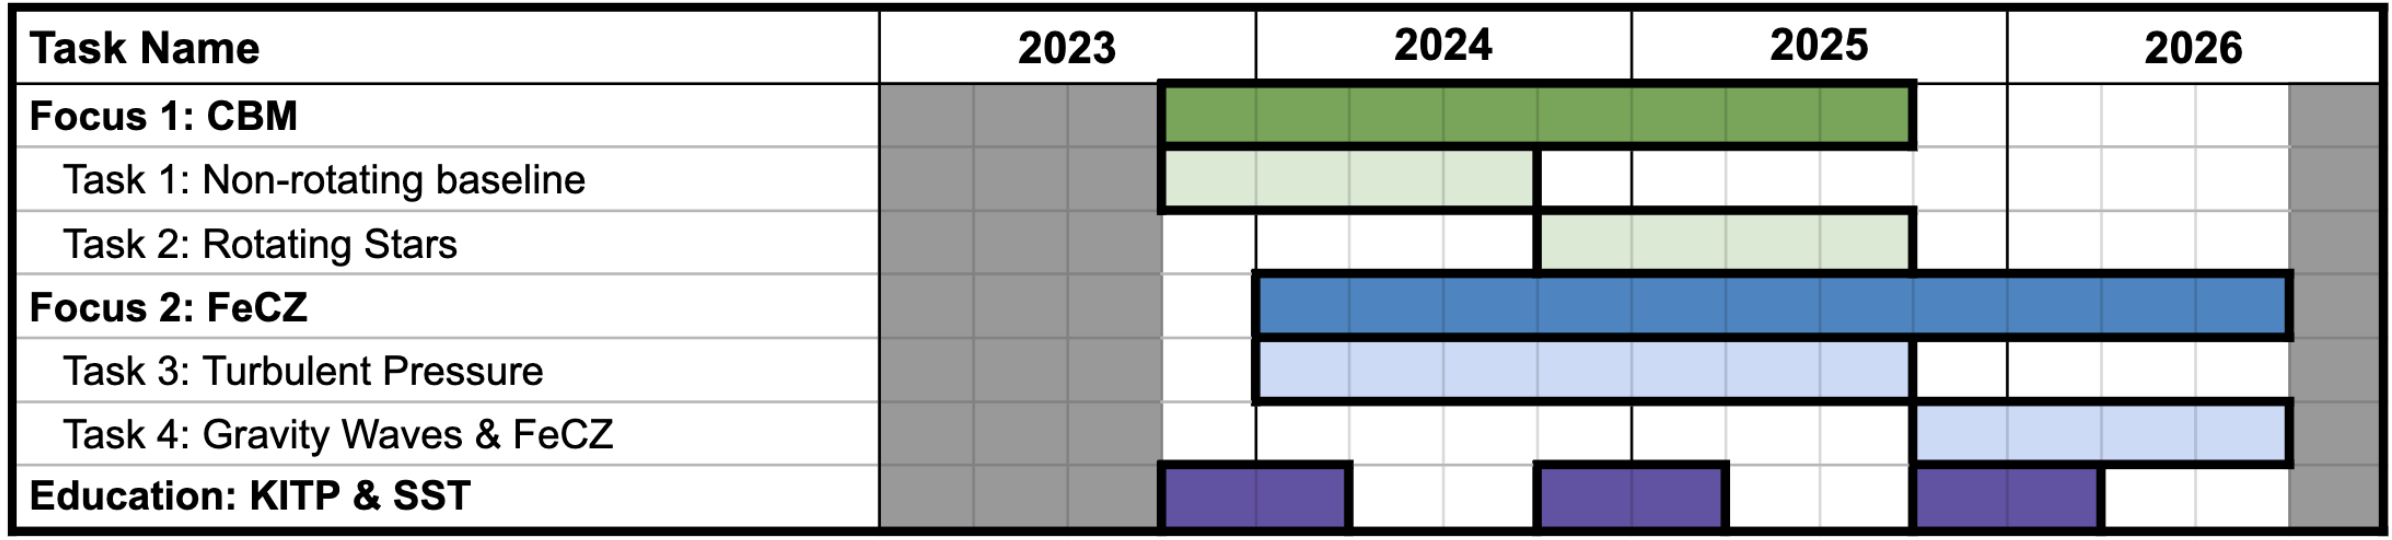
\includegraphics[width=\textwidth]{figures/gantt.png}
        \caption{A gantt diagram outlining the expected timeline of the proposed work. 
        \label{fig:gantt}}
\end{figure}

In Fig.~\ref{fig:gantt}, I lay out a timetable for the completion of the proposed activities.
Note that Focus I, Focus II, and my education plan will all happen in parallel.
Focus I and Focus II are functionally independent (one focuses on spherical simulations of low-Mach core convection, the other on Cartesian simulations of high-Mach FeCZ convection), so progress can be made on them in parallel.
I have spent much of the past year iterating and improving upon the \emph{Dedalus} implementation of the fully compressible equations in ball geometry, and on importing \emph{MESA} stellar models into \emph{Dedalus}, so I will be ready to run simulations and make progress on Task I immediately upon my arrival at KITP in fall 2023.
While these simulations are running, I will begin theory work and code design for the projects in focus II.
The research proposed here should result in at least four papers (two per focus, one per task), as well as open source community \emph{Dedalus} modules for simulating both spherical core convection and thin-shell FeCZ convection (in Cartesian).
SST module development will occur in the fall and winter quarter of each year, and the spring and summer will be reserved for iterating upon modules, publishing them, presenting them at conferences, and attending professional development workshops.

%%%%%%%%%%%%%%%%%%%%%%%%%%%%%%%%%%%%%%%%%%%%%%%%%%%%%%%%%%%%%%%%%%%%%%
\section{Reason for host institute choice}

KITP and UCSB are the ideal location for me to carry out this work.
By combining my expertise on convection and convective boundary mixing with the expertise of my proposed scientific mentor, Prof.~Lars Bildsten, on stellar structure, stellar evolution, and opacity-driven convection, we will be able to create the critical and timely simulations proposed here.
KITP is also the host institute of key \emph{MESA} developers like Prof.~Bildsten, so I will have access to the appropriate people when it comes time to implement my simulation-based prescriptions into stellar evolution software instruments.
Furthermore, KITP's scientific programs will bring experts to UCSB and KITP with whom I can collaborate, improve our theories, and understand additional problems that the proposed work can influence.
The opportunity to have KITP as a host institution at this early phase in my career will increase my cross section with leading experts from around the world and bolster my collaborative network.
I am particularly excited to participate in the ``Turbulence in Astrophysical Environments'' program in early 2024 and the ``Interconnections between the Physics of Plasmas and Self-gravitating Systems'' program in summer 2024.


\section{How the AAPF helps me achieve my career goals}
% -a description of the proposer's long term career goals and role of this postdoctoral experience in achieving them.

My career experiences have taught me that I love teaching, I love mentoring graduate student researchers, and I love participating in collaborative research projects which bridge gaps between disparate scientific sub-disciplines.
The only career path that will allow me to continue to participate in each of these activities is to become a professor at a research university, and that is my current career goal.
The work proposed in this fellowship will allow me to continue to build my identity as a scientist and gain further expertise developing and carrying out my own research plan, which is an essential part of being a professor.
Being located at KITP would allow me to interact with a diverse set of visiting scientists, exposing me to a wider range of exciting possible research avenues and providing me with numerous opportunities to form collaborations.
My proposed education plan will provide me with experience designing learning goals, crafting teaching plans, and facilitating activities in a classroom setting, all of which will be valuable experiences if I have the privilege to teach my own classes in the future.

\section{Relevance to Astro2020 Decadal Review goals}

This work will help answer two fundamental questions posed in the Astro2020 Decadal review: ``What [is] the mass ... distribution of neutron stars and stellar mass black holes?'' and ``What are the most extreme stars and stellar populations?''
This work will reduce error in core mixing prescriptions in stellar models, which can lead to errors in core mass estimates of order 70\% \citep{kaiser_etal_2020}.
These errors affect our ability to determine whether there is mass gap between black holes and neutron stars \citep{vanson_etal_2022} or where the boundaries of the pair instability black hole mass gap lie \citep{farmer_etal_2019}.
The mass of compact objects is one of their fundamental measurable properties, and stellar models provide theoretical constraints on expectations for observed mass distributions.
The proposed FeCZ simulations will lead to better estimates of stellar surface temperature thereby improving estimates of wind-driven mass loss.% and increasing our ability to model the effects of stellar feedback and evolution.


%%%%%%%%%%%%%%%%%%%%%%%%%%%%%%%%%%%%%%%%%%%%%%%%%%%%%%%%%%%%%%%%%%%%%%
\section*{Broader Impacts}

\textbf{This work will bolster scientific infrastructure in the field of stellar evolution and convection.}
Hydrodynamical simulations of 3D core convection are sparse, and the proposed work will create the first open-source tool for simulating 3D convection in the core of a massive star in the proper geometry and without any luminosity boosting; simulations studying convection spanning the full main-sequence will be produced and analyzed.
The results of these simulations will also be parameterized and integrated into the 1D MESA stellar evolution software instrument.
The proposed work will therefore create a new generation of 1D stellar evolution models which are informed by 3D turbulent convection and which can be compared with the growing wealth of precision astronomical observations.

\textbf{The proposed education plan focuses on broadening participation of underrepresented groups in the physical sciences.}
UCSB is a minority-serving institution and the SST interacts with a diverse set of high school students whose identities are underrepresented in my field.
By integrating my outreach plan with SST, I have the opportunity to provide young prospective scientists with a positive and authentic STEM experience.
By integrating my outreach plan with KITP programs, I can both tap into an international network of expert knowledge and create opportunities for wide distribution of my outreach materials.
%In summary, The proposed work will bolster recruitment of a diverse scientific workforce and have the possibility of international impact by employing instructors from a pool of scientists which spans the country and internationally.


% uncomment to include bibliography
%\newpage
%\setcounter{page}{1}
\bibliographystyle{unsrt}
\vfil\eject
\bibliography{biblio}

\end{document}